\chapter{三国演义}
    三国故事在中国民间流行久远。隋朝《大业拾遗记》记载隋炀帝观看曹操谯溪击蛟的杂戏,唐初,刘知几《史通》有“死诸葛能走生仲达”的故事。宋、元时代即被搬上舞台,孟元老的《东京梦华录》记载霍四究“说三分”之事。金、元演出的三国剧目达30多种。元英宗至治年间出现新安虞氏所刊的《全相三国志平话》。元末明初罗贯中综合民间传说和戏曲、话本,结合陈寿《三国志》和裴松之注的史料,根据他对社会人生的体悟,创作了《三国演义》。根据某些学者的考证,《三国演义》约在明代正统至景泰年间成书。

    三国演义的主要版本有:
    \begin{itemize}
        \item 明代嘉靖本《三国志通俗演义》
        \item 明代志传本《新刻按鉴全像批评三国志传》
        \item 明代李卓吾评本《李卓吾先生批评三国志》
        \item 清代李笠翁评本《李笠翁批阅三国志》
        \item 清代毛宗岗评改本《四大奇书第一种》
    \end{itemize}
    现存最早刊本是明朝嘉靖年刊刻的,俗称“嘉靖本”,全书24卷。亦有弘治刻本的《三国志通俗演义》,文字素朴,内容较平易。至清朝康熙年间,毛纶、毛宗岗父子辨正史事、增删文字,修改成今日通行的120回本《三国演义》,俗称“毛本”。

    近代较著名的校注本有吴小林《三国演义校注》,沈伯俊《校理本三国演义》。其中沈伯俊《校理本三国演义》,校正了原本中的大量“技术性错误”多达七八百处,得到国内外学术界同行的高度评价,并受到广大读者的欢迎,有人评论“迄今为止最好的《三国演义》版本”,被称为“沈本《三国演义》”,但也被批评有错误。
    滚滚长江东逝水,浪花淘尽英雄。是非成败转头空。青山依旧在,几度夕阳红。白发渔樵江渚上,惯看秋月春风。一壶浊酒喜相逢。古今多少事,都付笑谈中。——调寄《临江仙》
    \section{第一回\hspace{0.5em}宴桃园豪杰三结义\hspace{0.5em}斩黄巾英雄首立功}
        话说天下大势,分久必合,合久必分。周末七国分争,并入于秦。及秦灭之后,楚、汉分争,又并入于汉。汉朝自高祖斩白蛇而起义,一统天下,后来光武中兴,传至献帝,遂分为三国。推其致乱之由,殆始于桓、灵二帝。\ref{fig:one}桓帝禁锢善类,崇信宦官。及桓帝崩,灵帝即位,大将军窦武、太傅陈蕃共相辅佐。时有宦官曹节等弄权,窦武、陈蕃谋诛之,机事不密,反为所害,中涓自此愈横。
        \begin{figure}[h]
            \centering
            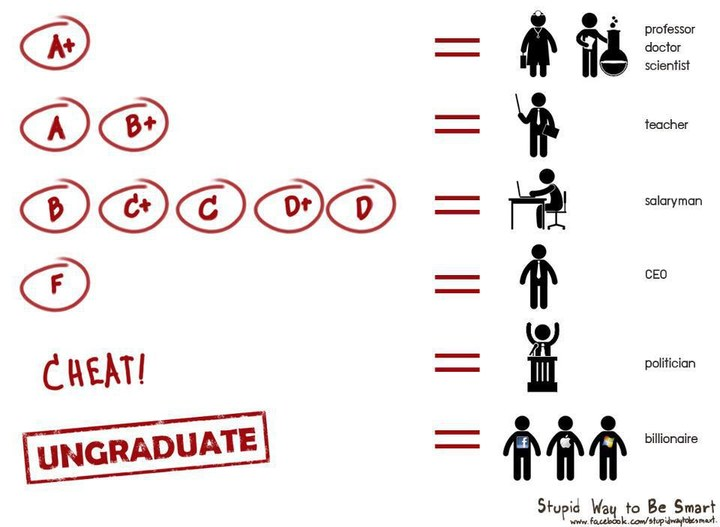
\includegraphics[scale=0.5]{grades.jpg}
            \caption{庄子语录}
            \label{fig:one}
        \end{figure}
        建宁二年四月望日,帝御温德殿。方升座,殿角狂风骤起。只见一条大青蛇,从梁上飞将下来,蟠于椅上。帝惊倒,左右急救入宫,百官俱奔避。须臾,蛇不见了。忽然大雷大雨,加以冰雹,落到半夜方止,坏却房屋无数。建宁四年二月,洛阳地震;又海水泛溢,沿海居民,尽被大浪卷入海中。光和元年,雌鸡化雄。六月朔,黑气十余丈,飞入温德殿中。秋七月,有虹现于玉堂;五原山岸,尽皆崩裂。种种不祥,非止一端。帝下诏问群臣以灾异之由,议郎蔡邕上疏,以为蝩堕鸡化,乃妇寺干政之所致,言颇切直。帝览奏叹息,因起更衣。曹节在后窃视,悉宣告左右;遂以他事陷邕于罪,放归田里。后张让、赵忠、封谞、段珪、曹节、侯览、蹇硕、程旷、夏恽、郭胜十人朋比为奸,号为“十常侍”。帝尊信张让,呼为“阿父”。朝政日非,以致天下人心思乱,盗贼蜂起。
    \section{第二回\hspace{0.5em}张翼德怒鞭督邮\hspace{0.5em}何国舅谋诛宦竖}
        且说董卓字仲颖,陇西临洮人也,官拜河东太守,自来骄傲。当日怠慢了玄德,张飞性发,便欲杀之。玄德与关公急止之曰;“他是朝廷命官,岂可擅杀?”飞曰:“若不杀这厮,反要在他部下听令,其实不甘!二兄要便住在此,我自投别处去也!”玄德曰:“我三人义同生死,岂可相离?不若都投别处去便了。”飞曰:“若如此,稍解吾恨。”

        于是三人连夜引军来投朱儁。儁待之甚厚,合兵一处,进讨张宝。是时曹操自跟皇甫嵩讨张梁,大战于曲阳。这里朱儁进攻张宝。张宝引贼众八九万,屯于山后。儁令玄德为其先锋,与贼对敌。张宝遣副将高升出马搦战,玄德使张飞击之。飞纵马挺矛,与升交战,不数合,刺升落马。玄德麾军直冲过去。张宝就马上披发仗剑,作起妖法。只见风雷大作,一股黑气从天而降,黑气中似有无限人马杀来。玄德连忙回军,军中大乱。败阵而归,与朱儁计议。儁曰:“彼用妖术,我来日可宰猪羊狗血,令军士伏于山头;候贼赶来,从高坡上泼之,其法可解。”玄德听令,拨关公、张飞各引军一千,伏于山后高冈之上,盛猪羊狗血并秽物准备。次日,张宝摇旗擂鼓,引军搦战,玄德出迎。交锋之际,张宝作法,风雷大作,飞砂走石,黑气漫天,滚滚人马,自天而下。玄德拨马便走,张宝驱兵赶来。将过山头,关、张伏军放起号炮,秽物齐泼。但见空中纸人草马,纷纷坠地;风雷顿息,砂石不飞。

        张宝见解了法,急欲退军。左关公,右张飞,两军都出,背后玄德、朱儁一齐赶上,贼兵大败。玄德望见“地公将军”旗号,飞马赶来,张宝落荒而走。玄德发箭,中其左臂。张宝带箭逃脱,走入阳城,坚守不出。
        \subsection{诗词节选}
            \hangindent=4em 汉朝天数当桓灵,炎炎红日将西倾。奸臣董卓废少帝,刘协懦弱魂梦惊。\\
            曹操传檄告天下,诸侯奋怒皆兴兵。议立袁绍作盟主,誓扶王室定太平。\\
            温侯吕布世无比,雄才四海夸英伟。护躯银铠砌龙鳞,束发金冠簪雉尾。\\
            参差宝带兽平吞,错落锦袍飞凤起。龙驹跳踏起天风,画戟荧煌射秋水。\\
            出关搦战谁敢当?诸侯胆裂心惶惶。踊出燕人张冀德,手持蛇矛丈八枪。\\
            虎须倒竖翻金线,环眼圆睁起电光。酣战未能分胜败,阵前恼起关云长。\\
            青龙宝刀灿霜雪,鹦鹉战袍飞蛱蝶。马蹄到处鬼神嚎,目前一怒应流血。\\
            枭雄玄德掣双锋,抖擞天威施勇烈。三人围绕战多时,遮拦架隔无休歇。\\
            喊声震动天地翻,杀气迷漫牛斗寒。吕布力穷寻走路,遥望家山拍马还。\\
            倒拖画杆方天戟,乱散销金五彩幡。顿断绒绦走赤兔,翻身飞上虎牢关。
